\documentclass[a4paper]{article}
\usepackage{graphicx}
\graphicspath{ {./img/} }

\newcommand{\wl}[1]{\textsf{\small #1}}

\begin{document}
\title{Computer Architecture Lab 3 Report}
\author{Fabian Wüthrich}
\date{November 2020}
\maketitle

\noindent
The task of this lab is to extend Ramulator to evaluate two memory scheduling
policies: ATLAS and BLISS. Before the actual implementation of the new
policies, the scheduler was refactored using the strategy design pattern to
make the code easier to extend. The refactoring removes many nested
if-statements and moves fields, that were only relevant to certain policies, to
the respective policy class.

\section*{Task 1: Implementing ATLAS}

For implementing ATLAS, we need to track for each thread the attained service
(AS) in the current quantum and the overall AS (TotalAS) up to the current quantum.
Ramulator executes only one thread per core, so \verb|coreid| is used
to identify a thread.

Each memory controller (see \verb|Controller.h|) tracks the AS of
a thread during a quantum in the vector \verb|attained_service|. When a request
is issued, the corresponding vector entry is incremented. Pending requests
occupy a bank for more cycles than normal requests. Thus, we increment the AS
counter for each pending request every cycle.

ATLAS requires a meta-controller to coordinate multiple memory controllers. The
meta-controller is implemented in the \verb|Memory| class because the class
has references to all memory controllers. At the end of a quantum, the
meta-controller accumulates the AS values for each thread (see line 295-302 in
\verb|Memory.h|). Then, the meta-controller recalculates the TotalAS for each
thread and passes the new value to all memory-controllers (see line 304-313).

The actual policy is implemented in \verb|Scheduler.h| by overriding the
\verb|compare()| function. The scheduler compares the arrival time of a request
to the clock count of the memory controller to figure out if the request has
been outstanding for more than T cycles (see line 229-233). If both requests are
below the threshold T, the scheduler queries the TotalAS value for each request
from the memory controller and picks the request with the lowest value (see line
235-241). If both AS values are the same, the scheduler prioritizes row hits and
then oldest requests first.

\newpage

\section*{Task 2: Implementing BLISS}

BLISS requires even less machinery than ATLAS and is implemented in
\verb|Controller.h|. The vector \verb|blacklisted| keeps track of the
blacklisted threads. Two variables (\verb|last_request_coreid| and
\verb|request_served_counter|) are used to identify malicious threads.

Similar to ATLAS the \verb|compare()| function is used to pick the best request.
The scheduler returns the request whose thread is not blacklisted or defaults to
row hits/oldest first if a decision based on the blacklist is not possible.

\section*{Task 3: Evaluation}

The evaluation compares ATLAS and BLISS to three scheduling policies (FCFS,
FRFCFS, FRFCFS\_Cap) which are already implemented in Ramulator. For each
scheduling policy, we simulated the following workloads:
\begin{itemize}
    \item Workload 1: \wl{HLLL} (four-core)
    \item Workload 2: \wl{HHLL} (four-core)
    \item Workload 3: \wl{HHHH} (four-core)
    \item Workload 4: \wl{HHHHHHHH} (eight-core)
\end{itemize}
where \texttt{H} stands for a workload with high memory intensity and \texttt{L}
is a workload with low memory intensity. Each simulation runs until every core
retires 20 million instructions. We evaluated the instruction throughput (IT)
and max. slowdown (MS), as defined in the lab sheet, for each workload using
each policy.

Figure \ref{fig:inst-throughput} shows the IT for each scheduling policy using
different workloads. \textbf{All policies have a similar IT for the two mixed
workloads} (9.5/7.1 instruction per cycles for \wl{HLLL}/\wl{HHLL}). The results
show more variation for the two intensive workloads (\wl{HHHH/HHHHHHHH}).
\textbf{ATLAS has the lowest performance} with 1.69 instructions per cycles on
average. \textbf{BLISS outperforms the other policies for the eight core
workloads} with 3.02 instructions per cycles.

Figure \ref{fig:max-slowdown} shows the MS for each policy. Similarly to the IT,
there are \textbf{no substantial differences for the two mixed workloads}. For
the \wl{HHHH} workload, the \textbf{MS increases for FCFS and ATLAS} to 1.19 and
1.47 respectively. For the eight core workload, \textbf{only BLISS is able to
keep the MS low} at 1.6 i.e.  guarantee fairness among the cores.

We expected that ATLAS outperforms the other policies for the mixed workloads
because threads with less attained service i.e. the \wl{L} workloads are
prioritized. Our simulation uses a system with just one memory controller and
four cores, whereas ATLAS was designed for multiple memory controllers in a many
core system, which explains the poor performance of ATLAS.

\newpage

The performance of ATLAS degrades significantly for the memory intensive
workloads (\wl{HHHH/HHHHHHHH}). This has primarily two reasons:
\begin{itemize}
    \item The \textbf{workloads are not optimal} to show the
        benefits of ATLAS. The simulation runs the same trace accessing the
        same addresses on four (eight) cores simultaneously. Such workloads
        are rare in practice and schedulers which prioritize row buffer
        locality i.e. FRFCFS, benefit from these workloads.

    \item ATLAS is a \textbf{unfair scheduling algorithm}, so instead of dividing
        the DRAM equally among all cores, requests of one core could be stalled for
        a long time degrading throughput.  This unfairness is also reflected in
        the MS for ATLAS. For the eight core workload, some cores are over 4x
        slower in a multi-core setting as when running alone on the system.
\end{itemize}

BLISS on the other hand is a \textbf{fair scheduling algorithm}. The MS for
BLISS running the eight-core workload is fairly low, whereas the unfairness of
the other scheduling algorithms increases. For the same reason, BLISS has
a better IT for the eight-core workload than the other scheduling policies.

\begin{figure}
    \centering
    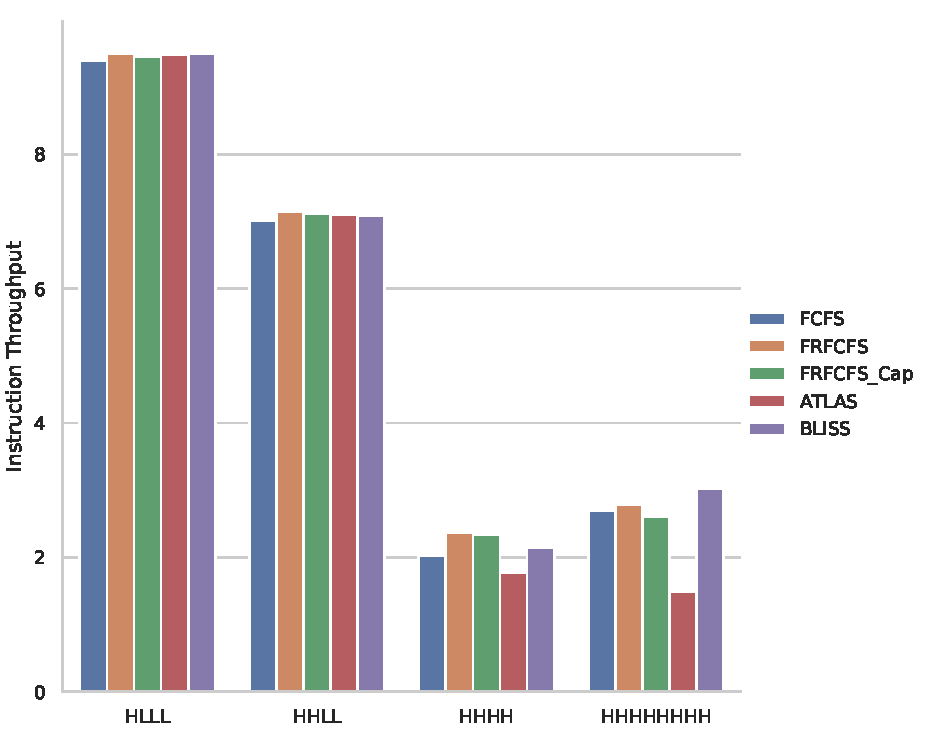
\includegraphics[width=\textwidth]{inst_throughput}
    \caption{Instruction Throughput}
    \label{fig:inst-throughput}
\end{figure}

\begin{figure}
    \centering
    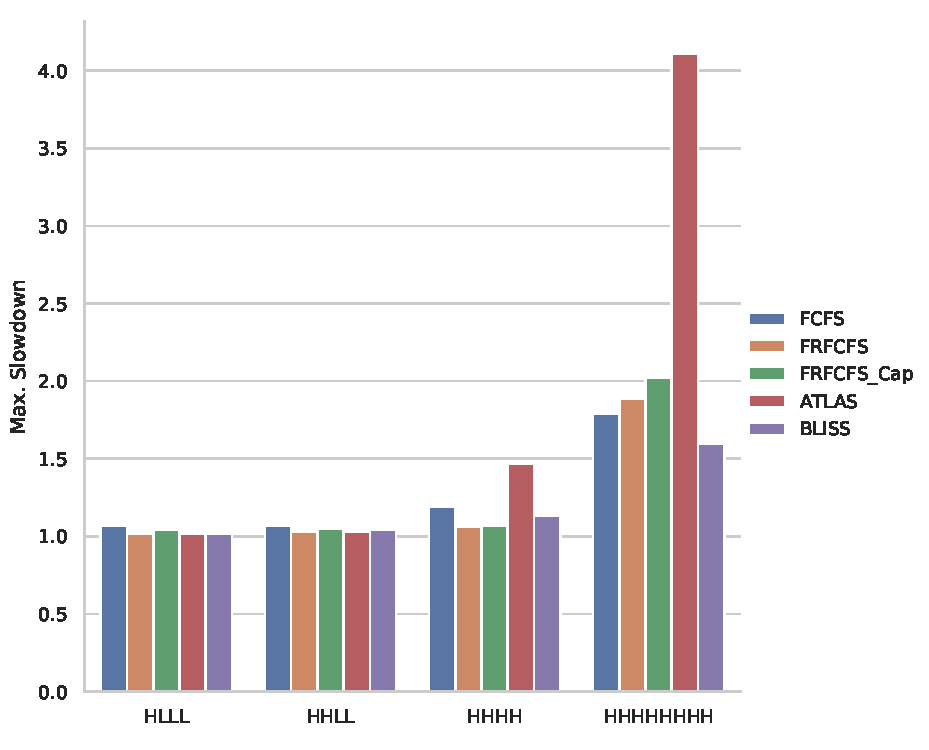
\includegraphics[width=\textwidth]{max_slowdown}
    \caption{Max. Slowdown}
    \label{fig:max-slowdown}
\end{figure}

\end{document}
